% !TEX program = xelatex
\documentclass[UTF8,zihao=-4,oneside,openany]{ctexbook}

\usepackage{graphicx}
\graphicspath{{assets/}}
% Shared style for the combined handout.  Section files keep standalone
% preambles for now, while the master document uses this single definition.
\usepackage[a4paper,top=20mm,bottom=22mm,left=19mm,right=19mm,headheight=24pt]{geometry}
\usepackage[table]{xcolor}
\usepackage{amsmath,amssymb,mathtools,bm}
\usepackage{siunitx}
\usepackage{booktabs,tabularx,array,multicol}
\usepackage{enumitem}
\usepackage{tikz}
\usetikzlibrary{arrows.meta,positioning,calc,angles,quotes,patterns}
\usepackage[most]{tcolorbox}
\usepackage{fancyhdr}
\usepackage{hyperref}

\definecolor{Ink}{HTML}{202326}
\definecolor{DeepBlue}{HTML}{294E69}
\definecolor{Blue}{HTML}{47687D}
\definecolor{PaleBlue}{HTML}{F3F5F6}
\definecolor{Gold}{HTML}{6E777D}
\definecolor{PaleGold}{HTML}{F6F6F5}
\definecolor{Green}{HTML}{5B6D76}
\definecolor{PaleGreen}{HTML}{F3F5F6}
\definecolor{Alert}{HTML}{666B6F}
\definecolor{PaleAlert}{HTML}{F6F6F6}
\definecolor{RuleGray}{HTML}{D3D7DA}
\definecolor{TextGray}{HTML}{61686D}
\definecolor{SoftGray}{HTML}{F6F6F6}

\color{Ink}
\sisetup{
  per-mode=symbol,
  inter-unit-product=\ensuremath{{}\cdot{}},
  exponent-product=\times
}

\hypersetup{
  colorlinks=true,
  linkcolor=DeepBlue,
  urlcolor=Blue,
  pdfsubject={高中物理竞赛一轮资料重排讲义},
  pdfauthor={物理竞赛一轮资料编写组}
}

\setlength{\parindent}{2em}
\setlength{\parskip}{0.25em}
\setlist{nosep,leftmargin=2em}
\setcounter{secnumdepth}{3}
\setcounter{tocdepth}{2}
\numberwithin{equation}{section}
\counterwithin{table}{section}
\allowdisplaybreaks[2]
\emergencystretch=2em

\ctexset{
  chapter={
    format=\raggedright\LARGE\bfseries\color{Ink},
    titleformat=\LARGE\bfseries\color{Ink},
    beforeskip=0pt,
    afterskip=18pt
  },
  section={
    format=\Large\bfseries\color{DeepBlue},
    beforeskip=1.8ex,
    afterskip=1.0ex
  },
  subsection={
    format=\large\bfseries\color{Ink},
    beforeskip=1.5ex,
    afterskip=0.8ex
  },
  subsubsection={format=\normalsize\bfseries\color{Ink}}
}

\pagestyle{fancy}
\fancyhf{}
\fancyhead[L]{\small\color{TextGray}高中物理竞赛一轮讲义}
\fancyhead[R]{\small\color{TextGray}第一章\quad 数学与物理工具}
\fancyfoot[C]{\small\color{TextGray}\thepage}
\renewcommand{\headrulewidth}{0.4pt}
\renewcommand{\headrule}{\hbox to\headwidth{\color{RuleGray}\leaders\hrule height \headrulewidth\hfill}}

\newcommand{\dimens}[1]{\operatorname{dim}\!\left(#1\right)}
\newcommand{\dd}{\mathop{}\!\mathrm{d}}
\newcommand{\vect}[1]{\bm{#1}}
\newcommand{\uvec}[1]{\hat{\vect{#1}}}
\newcommand{\e}{\mathrm e}
\newcommand{\order}[1]{\mathcal O\!\left(#1\right)}
\DeclareMathOperator{\proj}{proj}
\newcommand{\examplesource}[1]{%
  \par{\small\color{TextGray}题源：#1}\par
}

\newtcolorbox{goalbox}{
  enhanced,breakable,
  colback=PaleBlue,colframe=Blue,
  boxrule=0.7pt,arc=2mm,
  title={本节目标},fonttitle=\bfseries,
  coltitle=DeepBlue,
  attach boxed title to top left={xshift=5mm,yshift=-2mm},
  boxed title style={colback=white,colframe=Blue,boxrule=0.7pt,arc=1.5mm}
}

\newtcolorbox{sourcebox}{
  enhanced,breakable,
  colback=SoftGray,colframe=RuleGray,
  boxrule=0.5pt,arc=0mm,
  title={题源说明},fonttitle=\bfseries,
  coltitle=Ink,colbacktitle=SoftGray,
  borderline west={1.2pt}{0pt}{TextGray}
}

\newtcolorbox[auto counter,number within=section]{examplebox}[2][]{
  enhanced,breakable,
  colback=white,colframe=RuleGray,
  boxrule=0.5pt,arc=0mm,
  title={例题~\thetcbcounter\quad #2},fonttitle=\bfseries,
  coltitle=Ink,colbacktitle=PaleBlue,
  borderline west={1.4pt}{0pt}{DeepBlue},
  #1
}

\newtcolorbox{methodbox}[1]{
  enhanced,breakable,
  colback=PaleBlue,colframe=RuleGray,
  boxrule=0.5pt,arc=0mm,
  title={方法：#1},fonttitle=\bfseries,
  coltitle=Ink,colbacktitle=PaleBlue,
  borderline west={1.2pt}{0pt}{DeepBlue}
}

\newtcolorbox{warningbox}[1]{
  enhanced,breakable,
  colback=SoftGray,colframe=RuleGray,
  boxrule=0.5pt,arc=0mm,
  title={易错提醒：#1},fonttitle=\bfseries,
  coltitle=Ink,colbacktitle=SoftGray,
  borderline west={1.2pt}{0pt}{TextGray}
}

\newtcolorbox{extensionbox}[1]{
  enhanced,breakable,
  colback=PaleGold,colframe=Gold,
  boxrule=0.5pt,arc=0mm,
  title={拓展：#1},fonttitle=\bfseries,
  coltitle=Ink,colbacktitle=PaleGold,
  borderline west={1.2pt}{0pt}{DeepBlue}
}

\newtcolorbox{summarybox}{
  enhanced,breakable,
  colback=PaleBlue,colframe=DeepBlue,
  boxrule=0.9pt,arc=1.5mm,
  title={本节小结},fonttitle=\bfseries,
  coltitle=white,colbacktitle=DeepBlue
}

\newtcolorbox{exercisebox}[1]{
  enhanced,breakable,
  colback=white,colframe=RuleGray,
  boxrule=0.7pt,arc=1.5mm,
  title={#1},fonttitle=\bfseries,
  coltitle=DeepBlue,colbacktitle=PaleBlue
}

\tikzset{
  vector/.style={-{Latex[length=2.5mm]},very thick,draw=DeepBlue},
  component/.style={-{Latex[length=2.2mm]},thick,draw=TextGray},
  axis/.style={-{Latex[length=2mm]},thin,draw=TextGray},
  guide/.style={densely dashed,draw=TextGray},
  curve/.style={very thick,draw=DeepBlue},
  tangent/.style={thick,draw=TextGray},
  secant/.style={thick,draw=DeepBlue}
}

\usetikzlibrary{decorations.markings,decorations.pathmorphing,calc,arrows.meta,positioning,patterns,shapes.geometric}

\newcommand{\Needspace}[1]{%
  \par
  \ifdim\dimexpr\pagegoal-\pagetotal\relax<#1\relax
    \newpage
  \fi
}

\newtcolorbox{origexamplebox}[1]{
  enhanced,breakable,
  colback=white,colframe=RuleGray,
  boxrule=0.5pt,arc=0mm,
  title={#1},fonttitle=\bfseries,
  coltitle=Ink,colbacktitle=PaleBlue,
  borderline west={1.4pt}{0pt}{DeepBlue}
}

\NewDocumentEnvironment{xesolution}{+b}{%
  \par\smallskip
  \begingroup\small
  \noindent{\bfseries\color{DeepBlue}解答}\quad #1
  \par\endgroup\medskip
}{}

\hypersetup{
  pdftitle={高中物理竞赛一轮讲义：第35节 电介质、电容器（含解答与解图）},
  pdfsubject={依据学而思2020春高一物理第4讲完整整理，并补写推导、解答与解图},
  pdfauthor={原题资料：学而思；整理与解答：物理竞赛一轮资料编写组}
}

\fancyhead[R]{\small\color{TextGray}春季兴趣一阶\quad 第 4 讲}
\renewcommand{\theequation}{4.\arabic{equation}}

% Labels are deliberately transparent: no white boxes may cover geometry.
\tikzset{
  xeslabel/.style={font=\small,text=Ink,fill=none,inner sep=.55pt},
  xessmall/.style={font=\footnotesize,text=TextGray,fill=none,inner sep=.4pt},
  xestiny/.style={font=\scriptsize,text=TextGray,fill=none,inner sep=.3pt},
  xesline/.style={draw=Ink,line width=.85pt},
  xesblue/.style={draw=DeepBlue,line width=1pt},
  xesarrow/.style={-{Latex[length=2.1mm,width=1.3mm]},draw=DeepBlue,line width=.9pt},
  fieldline/.style={draw=DeepBlue,line width=.82pt,postaction={decorate},
    decoration={markings,mark=at position .57 with {\arrow{Latex[length=1.65mm,width=1.05mm]}}}},
  circuit/.style={draw=Ink,line width=.9pt,line cap=round,line join=round}
}

\newcommand{\diagramcaption}[1]{%
  \par\vspace{-.25em}
  \begin{center}\small\color{TextGray}#1\end{center}
  \vspace{.3em}
}

\newcommand{\capacitorFieldFigure}{%
\begin{center}
\includegraphics[width=.76\linewidth]{/Users/dongxingxi/Documents/物理竞赛一轮资料/sample/xes-original/restructured-complete/assets/revision-ch19-ch20/capacitor-pair.pdf}
\end{center}}


\newcommand{\parallelPlateFigure}{%
\begin{center}
\begin{tikzpicture}[x=1cm,y=1cm]
  % geometry panel
  \begin{scope}[shift={(-4.45,0)}]
    \fill[Gold!18] (-1.5,-1.25)--(-.72,-.85)--(-.72,1.25)--(-1.5,.85)--cycle;
    \draw[xesblue] (-1.5,-1.25)--(-.72,-.85)--(-.72,1.25)--(-1.5,.85)--cycle;
    \fill[DeepBlue!10] (.4,-1.25)--(1.18,-.85)--(1.18,1.25)--(.4,.85)--cycle;
    \draw[xesblue] (.4,-1.25)--(1.18,-.85)--(1.18,1.25)--(.4,.85)--cycle;
    \node[xeslabel,anchor=east] at (-1.58,.65) {$+Q$};
    \node[xeslabel,anchor=west] at (1.26,.65) {$-Q$};
    \draw[<->,Gold!80!black,line width=.65pt] (-.68,-1.55)--(.37,-1.55);
    \node[xestiny,text=Gold!70!black] at (-.15,-1.8) {$d$};
    \node[xessmall] at (0,1.65) {面积 $A$，板间距 $d$};
  \end{scope}
  \node[inner sep=0pt] at (3,0) {\includegraphics[width=6.7cm]{/Users/dongxingxi/Documents/物理竞赛一轮资料/sample/xes-original/restructured-complete/assets/revision-ch19-ch20/plate-edges.pdf}};

\end{tikzpicture}
\end{center}}

\newcommand{\coaxialCapacitorFigure}{%
\begin{center}
\begin{tikzpicture}[x=1cm,y=1cm]
  \begin{scope}[shift={(-3.0,0)}]
    \fill[DeepBlue!9] (-1.45,-1.55) rectangle (1.45,1.25);
    \draw[xesblue] (-1.45,-1.55)--(-1.45,1.25) (1.45,-1.55)--(1.45,1.25);
    \draw[xesblue] (0,1.25) ellipse (1.45 and .42);
    \draw[xesblue] (-1.45,-1.55) arc[start angle=180,end angle=360,x radius=1.45,y radius=.42];
    \fill[Gold!28] (-.62,-1.55) rectangle (.62,1.25);
    \draw[Gold!80!black,line width=.9pt] (-.62,-1.55)--(-.62,1.25) (.62,-1.55)--(.62,1.25);
    \draw[Gold!80!black,line width=.9pt] (0,1.25) ellipse (.62 and .2);
    \node[xessmall] at (0,-2.1) {同轴圆柱，长度 $h$};
    \draw[<->,Gold!75!black,line width=.6pt] (1.8,-1.55)--(1.8,1.25);
    \node[xestiny,text=Gold!70!black,anchor=west] at (1.95,-.15) {$h$};
  \end{scope}
  \begin{scope}[shift={(3.2,0)}]
    \fill[DeepBlue!8] (0,0) circle (1.65);
    
    \fill[Gold!26] (0,0) circle (.56);
    \draw[xesblue] (0,0) circle (1.65);
    \draw[Gold!80!black,line width=.9pt] (0,0) circle (.56);
    \foreach \a in {15,45,...,345}{\draw[fieldline] (\a:.62)--(\a:1.55);}
    \draw[Ink,line width=.55pt] (0,0)--(-.56,0);\node[xestiny,above] at (-.28,.05) {$a$};
    \draw[Ink,line width=.55pt] (0,0)--(1.65,0);\node[xestiny,below] at (1.12,-.04) {$b$};
    \node[xessmall] at (0,-2.1) {横截面：$a<r<b$};
  \end{scope}
\end{tikzpicture}
\end{center}}

\newcommand{\capacitorParallelFigure}{%
\begin{center}
\begin{tikzpicture}[x=1cm,y=1cm]
  \draw[circuit] (-3,-1.7)--(-3,1.7)--(-1.0,1.7);
  \draw[circuit] (1.0,1.7)--(3,1.7)--(3,-1.7);
  \draw[circuit] (-3,0)--(-1.0,0) (1.0,0)--(3,0);
  \draw[circuit] (-3,-1.7)--(-.45,-1.7) (.45,-1.7)--(3,-1.7);
  \draw[circuit,line width=1.4pt] (-1.0,1.42)--(-1.0,1.98) (1.0,1.42)--(1.0,1.98);
  \draw[circuit,line width=1.4pt] (-1.0,-.28)--(-1.0,.28) (1.0,-.28)--(1.0,.28);
  \draw[circuit,line width=1.4pt] (-.45,-2.08)--(-.45,-1.32) (.45,-1.94)--(.45,-1.46);
  \node[xeslabel,above] at (0,1.98) {$C_1$};
  \node[xeslabel,above] at (0,.28) {$C_2$};
  \node[xeslabel,below] at (0,-2.08) {$U$};
  \node[xessmall] at (0,1.15) {$Q_1=C_1U$};
  \node[xessmall] at (0,-.58) {$Q_2=C_2U$};
  \node[xessmall,align=left,anchor=west] at (4.0,.35) {两端电压相同\\总电荷相加};
\end{tikzpicture}
\end{center}}

\newcommand{\capacitorSeriesFigure}{%
\begin{center}
\begin{tikzpicture}[x=1cm,y=1cm]
  \draw[circuit] (-3,-1.45)--(-3,1.45)--(-1.55,1.45);
  \draw[circuit] (-.75,1.45)--(.75,1.45);
  \draw[circuit] (1.55,1.45)--(3,1.45)--(3,-1.45);
  \draw[circuit] (-3,-1.45)--(-.45,-1.45) (.45,-1.45)--(3,-1.45);
  \draw[circuit,line width=1.4pt] (-1.55,1.17)--(-1.55,1.73) (-.75,1.17)--(-.75,1.73);
  \draw[circuit,line width=1.4pt] (.75,1.17)--(.75,1.73) (1.55,1.17)--(1.55,1.73);
  \draw[circuit,line width=1.4pt] (-.45,-1.83)--(-.45,-1.07) (.45,-1.69)--(.45,-1.21);
  \node[xeslabel,above] at (-1.15,1.76) {$C_1$};
  \node[xeslabel,above] at (1.15,1.76) {$C_2$};
  \node[xeslabel,below] at (0,-1.87) {$U$};
  \node[xessmall,align=center] at (0,.55) {中间导体净电荷为零\\两电容电荷量均为 $Q$};
  \node[xessmall] at (0,-.45) {$U=Q/C_1+Q/C_2$};
\end{tikzpicture}
\end{center}}

\newcommand{\greenSphereFigure}{%
\begin{center}
\begin{tikzpicture}[x=1cm,y=1cm]
  \fill[Gold!16] (-1.3,0) circle (1.25);\draw[xesblue] (-1.3,0) circle (1.25);
  \fill[Ink] (3.35,0) circle (2.2pt);\node[xeslabel,above=4pt] at (3.35,0) {$P$};
  \fill[Ink] (-1.3,0) circle (1.7pt);
  \draw[xesline] (-1.3,0)--(3.35,0);
  \node[xeslabel,above] at (1.0,0) {$r$};
  \node[xessmall,align=left,anchor=west] at (4.25,.35) {状态 A：球带单位电荷\\状态 B：$P$ 点放电荷 $q$};
\end{tikzpicture}
\end{center}}

\newcommand{\greenTwoConductorFigure}{%
\begin{center}
\begin{tikzpicture}[x=1cm,y=1cm]
  \fill[DeepBlue!10] (-2.6,0) ellipse (1.3 and .95);\draw[xesblue] (-2.6,0) ellipse (1.3 and .95);
  \fill[Gold!16] (2.4,.1) ellipse (1.05 and 1.18);\draw[xesblue] (2.4,.1) ellipse (1.05 and 1.18);
  \node[xeslabel,align=center] at (-2.6,0) {$Q_1$\\$\varphi_1$};
  \node[xeslabel,align=center] at (2.4,.1) {$Q_2$\\$\varphi_2$};
  \draw[<->,Gold!75!black,line width=.65pt] (-1.15,0)--(1.2,0);
  \node[xessmall,text=Gold!70!black,above] at (0,.05) {静电感应耦合};
  \node[xessmall] at (0,-1.55) {另一状态用 $Q'_i,\varphi'_i$ 表示，几何形状保持不变};
\end{tikzpicture}
\end{center}}

\newcommand{\dielectricMeterFigure}{%
\begin{center}
\includegraphics[width=.93\linewidth]{/Users/dongxingxi/Documents/物理竞赛一轮资料/sample/xes-original/restructured-complete/assets/revision-ch19-ch20/dielectric-meter.png}
\end{center}}


\newcommand{\polarizationFigure}{%
\begin{center}
\begin{tikzpicture}[x=1cm,y=1cm]
  \begin{scope}[shift={(-3.6,0)}]
    \draw[xesblue] (-2.1,-1.45) rectangle (2.1,1.45);
    \foreach \x in {-1.45,0,1.45}{\foreach \y in {-0.85,0,.85}{
      \fill[DeepBlue!20] (\x-.24,\y) ellipse (.38 and .2);
      \fill[Gold!35] (\x+.24,\y) ellipse (.38 and .2);
      \node[xestiny,text=Ink] at (\x-.28,\y) {$-$};
      \node[xestiny,text=Ink] at (\x+.28,\y) {$+$};}}
    \draw[xesarrow] (-1.8,1.9)--(1.8,1.9);
    \node[xessmall,above] at (0,1.93) {$\boldsymbol E_0$};
    \node[xessmall] at (0,-1.8) {微观：偶极矩沿外场排列};
  \end{scope}
  \begin{scope}[shift={(3.6,0)}]
    \draw[xesblue] (-2.1,-1.45) rectangle (2.1,1.45);
    \foreach \y in {-1.1,-.55,0,.55,1.1}{
      \node[xestiny,text=Ink] at (-1.82,\y) {$-$};
      \node[xestiny,text=Ink] at (1.82,\y) {$+$};
      \draw[-{Latex[length=1.65mm]},Gold!80!black,line width=.72pt] (1.35,\y)--(-1.35,\y);}
    \node[xessmall,text=Gold!70!black] at (0,.28) {$\boldsymbol E_p$};
    \node[xessmall] at (0,-1.8) {宏观：束缚面电荷产生反向极化场};
    \node[xestiny,anchor=east] at (-2.25,0) {$-\sigma_p$};
    \node[xestiny,anchor=west] at (2.25,0) {$+\sigma_p$};
  \end{scope}
\end{tikzpicture}
\end{center}}

\newcommand{\exampleParallelFigure}{%
\begin{center}
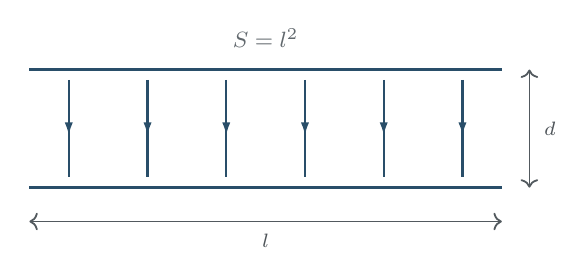
\begin{tikzpicture}[x=1cm,y=1cm]
  \draw[xesblue,line width=1.25pt] (-3,.75)--(3,.75);
  \draw[xesblue,line width=1.25pt] (-3,-.75)--(3,-.75);
  \draw[<->,Gold!75!black,line width=.65pt] (3.35,-.75)--(3.35,.75);
  \node[xestiny,text=Gold!70!black,anchor=west] at (3.52,0) {$d$};
  \draw[<->,Gold!75!black,line width=.65pt] (-3,-1.18)--(3,-1.18);
  \node[xestiny,text=Gold!70!black] at (0,-1.42) {$l$};
  \node[xessmall] at (0,1.15) {$S=l^2$};
  \foreach \x in {-2.5,-1.5,...,2.5}{\draw[fieldline] (\x,.62)--(\x,-.62);}
\end{tikzpicture}
\end{center}}

\newcommand{\exampleSphericalFigure}{%
\begin{center}
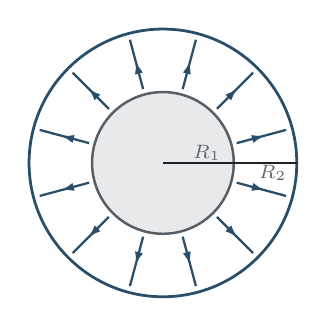
\begin{tikzpicture}[x=1cm,y=1cm]
  
  \fill[Gold!16] (0,0) circle (.9);
  \draw[xesblue] (0,0) circle (1.7);
  \draw[Gold!80!black,line width=.9pt] (0,0) circle (.9);
  \draw[xesline] (0,0)--(.9,0) node[xestiny,pos=.62,above] {$R_1$};
  \draw[xesline] (0,0)--(1.7,0) node[xestiny,pos=.82,below] {$R_2$};
  \foreach \a in {15,45,...,345}{\draw[fieldline] (\a:.97)--(\a:1.62);}
\end{tikzpicture}
\end{center}}

\newcommand{\touchingSpheresFigure}{%
\begin{center}
\begin{tikzpicture}[x=1cm,y=1cm]
  \fill[DeepBlue!7] (-1.25,0) circle (1.25);\draw[xesblue] (-1.25,0) circle (1.25);
  \fill[DeepBlue!7] (1.25,0) circle (1.25);\draw[xesblue] (1.25,0) circle (1.25);
  \draw[xesline] (1.25,0)--(2.13,.88);
  \node[xeslabel,above] at (1.72,.48) {$R$};
  \node[xessmall] at (0,-1.65) {两球接触并处于同一电势 $V$};
\end{tikzpicture}
\end{center}}

\newcommand{\touchingSphereImagesFigure}{%
\begin{center}
\begin{tikzpicture}[x=1cm,y=1cm]
  \draw[xesblue] (-1.55,0) circle (1.55);\draw[xesblue] (1.55,0) circle (1.55);
  \draw[RuleGray,densely dashed,line width=.55pt] (-3.2,0)--(3.2,0);
  \foreach \x/\sgn in {-1.55/DeepBlue,-.78/Ink,-.52/DeepBlue,-.39/Ink,
                         1.55/DeepBlue,.78/Ink,.52/DeepBlue,.39/Ink}{
    \fill[\sgn] (\x,0) circle (3.1pt);}
  % 接触点附近的像电荷十分密集；用错层引线避免 q_2,q_3,q_4 互相覆盖。
  \node[xestiny,above=3pt] at (-1.55,0) {$q_1$};
  \draw[RuleGray,line width=.45pt] (-.78,-.05)--(-.90,-.34)
    node[xestiny,below] {$q_2$};
  \draw[RuleGray,line width=.45pt] (-.52,.05)--(-.70,.38)
    node[xestiny,above] {$q_3$};
  \draw[RuleGray,line width=.45pt] (-.39,-.05)--(-.48,-.64)
    node[xestiny,below] {$q_4$};
  \node[xestiny,above=3pt] at (1.55,0) {$q_1$};
  \draw[RuleGray,line width=.45pt] (.78,-.05)--(.90,-.34)
    node[xestiny,below] {$q_2$};
  \draw[RuleGray,line width=.45pt] (.52,.05)--(.70,.38)
    node[xestiny,above] {$q_3$};
  \draw[RuleGray,line width=.45pt] (.39,-.05)--(.48,-.64)
    node[xestiny,below] {$q_4$};
  \node[xessmall] at (0,-1.95) {$x_n=R/n,\quad q_n=4\pi\varepsilon_0RV\,(-1)^{n-1}/n$};
  \node[xessmall] at (0,-2.43) {两侧电荷序列都向接触点聚集};
\end{tikzpicture}
\end{center}}

\newcommand{\twoCylindersFigure}{%
\begin{center}
\includegraphics[width=.76\linewidth]{/Users/dongxingxi/Documents/物理竞赛一轮资料/sample/xes-original/restructured-complete/assets/revision-ch19-ch20/two-cylinders.pdf}
\end{center}}


\newcommand{\modifiedCapacitorFigure}{%
\begin{center}
\begin{tikzpicture}[x=1cm,y=1cm]
  \begin{scope}[shift={(-3.5,0)}]
    \draw[xesblue,line width=1.1pt] (-2,1)--(2,1) (-2,-1)--(2,-1);
    \fill[Gold!22,pattern=north east lines,pattern color=Gold!70!black] (-2,-.9) rectangle (0,.9);
    \draw[RuleGray,line width=.55pt] (0,-.9)--(0,.9);
    \node[xessmall] at (-1,0) {$\varepsilon_r$};\node[xessmall] at (1,0) {真空};
    \node[xessmall] at (0,-1.42) {(a) 占一半面积：两个电容并联};
  \end{scope}
  \begin{scope}[shift={(3.5,0)}]
    \draw[xesblue,line width=1.1pt] (-2,1)--(2,1) (-2,-1)--(2,-1);
    \fill[Gold!22,pattern=north east lines,pattern color=Gold!70!black] (-2,0) rectangle (2,.9);
    \draw[RuleGray,line width=.55pt] (-2,0)--(2,0);
    \node[xessmall] at (0,.45) {$\varepsilon_r$};\node[xessmall] at (0,-.48) {真空};
    \node[xessmall] at (0,-1.42) {(b) 占一半厚度：两个电容串联};
  \end{scope}
\end{tikzpicture}
\end{center}}

\newcommand{\dielectricInsertionFigure}{%
\begin{center}
\begin{tikzpicture}[x=1cm,y=1cm]
  \draw[xesblue,line width=1.2pt] (-4,1)--(4,1) (-4,-1)--(4,-1);
  \fill[Gold!22,pattern=north east lines,pattern color=Gold!70!black] (-4,-.9) rectangle (1.0,.9);
  \draw[Gold!80!black,line width=.75pt] (1.0,-.9)--(1.0,.9);
  \draw[<->,Gold!75!black,line width=.65pt] (-4,1.38)--(1.0,1.38);
  \node[xestiny,text=Gold!70!black] at (-1.5,1.62) {$x$};
  \draw[<->,Gold!75!black,line width=.65pt] (1.0,1.38)--(4,1.38);
  \node[xestiny,text=Gold!70!black] at (2.5,1.62) {$a-x$};
  \draw[<->,Gold!75!black,line width=.65pt] (4.35,-1)--(4.35,1);
  \node[xestiny,text=Gold!70!black,anchor=west] at (4.5,0) {$d$};
  \draw[xesarrow] (.6,0)--(1.75,0);\node[xessmall,above] at (1.18,.05) {$F$};
  \node[xessmall] at (-1.5,0) {$\varepsilon_r$};
  \node[xessmall] at (0,-1.48) {极板宽度为 $b$，总面积 $S=ab$};
\end{tikzpicture}
\end{center}}

\newcommand{\yCapacitorFigure}{%
\begin{center}
\begin{tikzpicture}[x=1cm,y=1cm]
  \coordinate (O) at (0,0);
  \draw[circuit] (O)--(0,.62);
  \draw[circuit,line width=1.35pt] (-.34,.62)--(.34,.62) (-.34,1.02)--(.34,1.02);
  \draw[circuit] (0,1.02)--(0,1.85);
  \node[xeslabel,anchor=west] at (.45,.82) {$C_1$};\node[xeslabel,above] at (0,1.85) {$\varphi_1$};
  \begin{scope}[rotate=120]
    \draw[circuit] (0,0)--(0,.72);
    \draw[circuit,line width=1.35pt] (-.34,.72)--(.34,.72) (-.34,1.12)--(.34,1.12);
    \draw[circuit] (0,1.12)--(0,1.95);
  \end{scope}
  \node[xeslabel] at (-1.85,-1.18) {$\varphi_2$};\node[xeslabel] at (-1.00,-1.02) {$C_2$};
  \begin{scope}[rotate=-120]
    \draw[circuit] (0,0)--(0,.72);
    \draw[circuit,line width=1.35pt] (-.34,.72)--(.34,.72) (-.34,1.12)--(.34,1.12);
    \draw[circuit] (0,1.12)--(0,1.95);
  \end{scope}
  \node[xeslabel] at (1.85,-1.18) {$\varphi_3$};\node[xeslabel] at (1.00,-1.02) {$C_3$};
  \fill[DeepBlue] (O) circle (2.3pt);\node[xessmall,anchor=west] at (.18,.12) {浮置中性节点，电势 $V$};
\end{tikzpicture}
\end{center}}

\newcommand{\dielectricSphereFieldFigure}{%
\begin{center}
\includegraphics[width=.76\linewidth]{/Users/dongxingxi/Documents/物理竞赛一轮资料/sample/xes-original/restructured-complete/assets/revision-ch19-ch20/dielectric-sphere.pdf}
\end{center}}


\newcommand{\polarizationEnergyFigure}{%
\begin{center}
\begin{tikzpicture}[x=1cm,y=1cm]
  \begin{scope}[shift={(-3.3,0)}]
    \draw[xesblue] (-1.7,-1.0) rectangle (1.7,1.0);
    \foreach \x in {-1.15,0,1.15}{\draw[decorate,decoration={zigzag,segment length=3pt,amplitude=2pt},Gold!75!black,line width=.7pt] (\x-.35,0)--(\x+.35,0);}
    \foreach \x in {-1.15,0,1.15}{\node[xestiny] at (\x-.48,0) {$-$};\node[xestiny] at (\x+.48,0) {$+$};}
    \node[xessmall] at (0,-1.38) {无外场：微观“弹簧”未拉伸};
  \end{scope}
  \begin{scope}[shift={(3.3,0)}]
    \draw[xesblue] (-1.7,-1.0) rectangle (1.7,1.0);
    \foreach \x in {-1.15,0,1.15}{\draw[decorate,decoration={zigzag,segment length=3pt,amplitude=2pt},Gold!75!black,line width=.7pt] (\x-.55,0)--(\x+.55,0);}
    \foreach \x in {-1.15,0,1.15}{\node[xestiny] at (\x-.7,0) {$-$};\node[xestiny] at (\x+.7,0) {$+$};}
    \draw[xesarrow] (-1.45,.68)--(1.45,.68);\node[xessmall,above] at (0,.71) {$\boldsymbol E$};
    \node[xessmall] at (0,-1.38) {有外场：极化自由度也储存能量};
  \end{scope}
\end{tikzpicture}
\end{center}}

\newcommand{\chargingEnergyFigure}{%
\begin{center}
\begin{tikzpicture}[x=1cm,y=1cm]
  \node[draw=DeepBlue,line width=.9pt,rounded corners=2pt,minimum width=2.3cm,minimum height=1.0cm,text=Ink,fill=DeepBlue!6] (S) at (-3.6,0) {电源 $C\mathcal E^2$};
  \node[draw=DeepBlue,line width=.9pt,rounded corners=2pt,minimum width=2.4cm,minimum height=1.0cm,text=Ink,fill=DeepBlue!6] (C) at (0,1.15) {电容场能 $\tfrac12C\mathcal E^2$};
  \node[draw=Gold!80!black,line width=.9pt,rounded corners=2pt,minimum width=2.4cm,minimum height=1.0cm,text=Ink,fill=Gold!12] (H) at (0,-1.15) {焦耳热 $\tfrac12C\mathcal E^2$};
  \draw[xesarrow] (S.east)--(C.west);\draw[-{Latex[length=2.1mm]},Gold!80!black,line width=.9pt] (S.east)--(H.west);
  \node[xessmall,align=left,anchor=west] at (2.1,.25) {$R>0$ 时分配比例与 $R$ 无关；\\$R\to0^+$ 只使过程更快。};
\end{tikzpicture}
\end{center}}

\newcommand{\earthCapacitorFigure}{%
\begin{center}
\begin{tikzpicture}[x=1cm,y=1cm]
  \fill[DeepBlue!16] (0,0) circle (2.05);\draw[xesblue] (0,0) circle (2.05);
  \draw[Gold!80!black,line width=3.3pt,opacity=.7] (0,0) circle (2.34);
  \node[xessmall] at (0,0) {地球};
  \node[xestiny] at (0,-.45) {半径 $R_\oplus$，电荷 $-Q$};
  \draw[<->,Gold!75!black,line width=.65pt] (2.05,0)--(2.34,0);
  \node[xestiny,text=Gold!70!black,anchor=west] at (2.48,0) {$d=5\,\mathrm{km}$};
  \node[xessmall,anchor=west] at (3.35,.62) {等效大气上边界：$+Q$};
  \draw[RuleGray,-{Latex[length=1.5mm]},line width=.55pt] (3.2,.55)--(2.25,.35);
  \node[xessmall,anchor=west] at (3.35,-.35) {$C=4\pi\varepsilon_0\dfrac{R_\oplus(R_\oplus+d)}{d}$};
\end{tikzpicture}
\end{center}}

% Pure question geometry; analysis figure retained separately.
\newcommand{\emParallelQuestion}{%
\begin{center}
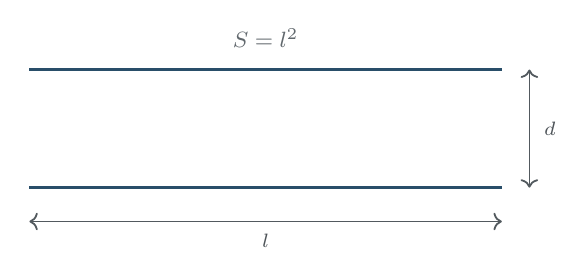
\begin{tikzpicture}[x=1cm,y=1cm]
  \draw[xesblue,line width=1.25pt] (-3,.75)--(3,.75);
  \draw[xesblue,line width=1.25pt] (-3,-.75)--(3,-.75);
  \draw[<->,Gold!75!black,line width=.65pt] (3.35,-.75)--(3.35,.75);
  \node[xestiny,text=Gold!70!black,anchor=west] at (3.52,0) {$d$};
  \draw[<->,Gold!75!black,line width=.65pt] (-3,-1.18)--(3,-1.18);
  \node[xestiny,text=Gold!70!black] at (0,-1.42) {$l$};
  \node[xessmall] at (0,1.15) {$S=l^2$};
\end{tikzpicture}
\end{center}}

% Pure question geometry; analysis figure retained separately.
\newcommand{\emSphericalQuestion}{%
\begin{center}
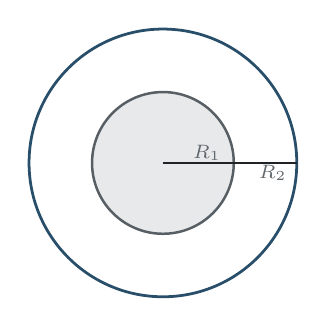
\begin{tikzpicture}[x=1cm,y=1cm]
  
  \fill[Gold!16] (0,0) circle (.9);
  \draw[xesblue] (0,0) circle (1.7);
  \draw[Gold!80!black,line width=.9pt] (0,0) circle (.9);
  \draw[xesline] (0,0)--(.9,0) node[xestiny,pos=.62,above] {$R_1$};
  \draw[xesline] (0,0)--(1.7,0) node[xestiny,pos=.82,below] {$R_2$};
\end{tikzpicture}
\end{center}}

% Pure question geometry; analysis figure retained separately.
\newcommand{\emModifiedQuestion}{%
\begin{center}
\begin{tikzpicture}[x=1cm,y=1cm]
  \path[use as bounding box] (-5.55,-1.7) rectangle (5.55,1.15);
  \begin{scope}[shift={(-3.5,0)}]
    \fill[Gold!22,pattern=north east lines,pattern color=Gold!70!black] (-2,-.9) rectangle (0,.9);
    \draw[RuleGray,line width=.55pt] (0,-.9)--(0,.9);
    \node[xessmall] at (-1,0) {$\varepsilon_r$};\node[xessmall] at (1,0) {真空};
    \draw[xesblue,line width=1.1pt] (-2,1)--(2,1) (-2,-1)--(2,-1);
    \node[xessmall] at (0,-1.42) {(a) 占一半面积};
  \end{scope}
  \begin{scope}[shift={(3.5,0)}]
    \fill[Gold!22,pattern=north east lines,pattern color=Gold!70!black] (-2,0) rectangle (2,.9);
    \draw[RuleGray,line width=.55pt] (-2,0)--(2,0);
    \node[xessmall] at (0,.45) {$\varepsilon_r$};\node[xessmall] at (0,-.48) {真空};
    \draw[xesblue,line width=1.1pt] (-2,1)--(2,1) (-2,-1)--(2,-1);
    \node[xessmall] at (0,-1.42) {(b) 占一半厚度};
  \end{scope}
\end{tikzpicture}
\end{center}}

% Pure question geometry; analysis figure retained separately.
\newcommand{\emInsertionQuestion}{%
\begin{center}
\begin{tikzpicture}[x=1cm,y=1cm]
  \draw[xesblue,line width=1.2pt] (-4,1)--(4,1) (-4,-1)--(4,-1);
  \fill[Gold!22,pattern=north east lines,pattern color=Gold!70!black] (-4,-.9) rectangle (1.0,.9);
  \draw[Gold!80!black,line width=.75pt] (1.0,-.9)--(1.0,.9);
  \draw[<->,Gold!75!black,line width=.65pt] (-4,1.38)--(1.0,1.38);
  \node[xestiny,text=Gold!70!black] at (-1.5,1.62) {$x$};
  \draw[<->,Gold!75!black,line width=.65pt] (1.0,1.38)--(4,1.38);
  \node[xestiny,text=Gold!70!black] at (2.5,1.62) {$a-x$};
  \draw[<->,Gold!75!black,line width=.65pt] (4.35,-1)--(4.35,1);
  \node[xestiny,text=Gold!70!black,anchor=west] at (4.5,0) {$d$};
  \node[xessmall] at (-1.5,0) {$\varepsilon_r$};
  \node[xessmall] at (0,-1.48) {极板宽度为 $b$，总面积 $S=ab$};
\end{tikzpicture}
\end{center}}


\begin{document}
\pagenumbering{arabic}
\setcounter{page}{1}
\setcounter{equation}{0}

\section*{第 4 讲\quad 电介质、电容器}

上一讲讨论了导体在静电平衡状态下的性质：导体内部电场为零，整个导体是等势体，电荷分布在表面。
当几个导体共同存在时，每个导体都可以用其电荷和电势描述；改变一个导体的电荷，还会通过静电感应
改变其他导体的表面电荷分布与电势。本讲把这种相互作用定量化。最简单的量是孤立导体的电容以及由
两个导体构成的电容器的电容；在此基础上，还要讨论一般导体组、介质极化和电位移矢量。

\subsection*{孤立导体的电容}

先设想空间中有许多导体，其中只有一个导体不接地，其余导体均与大地相连，电势固定为零。给这个
孤立导体电荷 $Q$ 后，它达到静电平衡并具有电势 $U$。由静电场的唯一性和叠加原理可知：导体的几何
形状、位置及周围接地边界不变时，把所有电荷同时放大 $k$ 倍，电势也放大 $k$ 倍。因此 $Q$ 与 $U$
成正比，写成
\begin{equation}
  \boxed{Q=CU}.
\end{equation}
比例系数 $C$ 称为该孤立导体的电容。它只由导体的形状、大小、位置以及周围边界决定，与本次给它多少
电荷无关。在国际单位制中电容的单位是法拉，$1\,\mathrm F=1\,\mathrm C/\mathrm V$；实际孤立导体的
电容通常很小，常用 $\mu\mathrm F$、$\mathrm{nF}$ 和 $\mathrm{pF}$。

半径为 $R$ 的孤立导体球外没有其他导体。球带电 $Q$ 时，球面外电场与位于球心的点电荷相同，取无穷远
电势为零，球面电势为
\[
  U=\int_R^{\infty}\frac{Q}{4\pi\varepsilon_0r^2}\,\mathrm dr
   =\frac{Q}{4\pi\varepsilon_0R}.
\]
代入定义得到
\begin{equation}
  \boxed{C=\frac QU=4\pi\varepsilon_0R}.
\end{equation}
可见球半径越大，达到相同电势所需的电荷越多，电容也越大。例如 $R=1\,\mathrm m$ 时，电容仍只有
约 $111\,\mathrm{pF}$。

若孤立导体的电容为 $C$，把它从不带电缓慢充到电荷 $Q$。中间状态带电 $q$ 时电势为 $q/C$，再搬入
$\mathrm dq$ 所做的功为 $(q/C)\mathrm dq$。总静电能为
\begin{equation}
  \boxed{W=\int_0^Q\frac qC\,\mathrm dq
  =\frac{Q^2}{2C}=\frac12QU=\frac12CU^2}.
\end{equation}
这些能量保存在导体带电所建立的电场中。由于静电场能量密度非负，电容也必为正数。

\subsection*{电容器的电容}

取两个彼此绝缘的导体，分别带 $+Q$ 和 $-Q$。若它们的放置使电场主要限制在两者之间，这一导体组
称为电容器，两个导体称为两极。带正电的一极为正极，另一极为负极。

图 4.1 以两球为例，正球上的场线沿外法线发出，负球上的场线沿内法线进入；两球各自等势，但电势一般不同。

\capacitorFieldFigure
\diagramcaption{图 4.1：双极电容器的两球示例。两极带等量异号电荷，电场线由正极指向负极。}

由唯一性定理，两极电荷量 $Q$ 与电势差 $U=\varphi_+-\varphi_-$ 成正比：
\begin{equation}
  \boxed{Q=CU}.
\end{equation}
这里的 $C$ 是电容器的电容量。孤立导体与双极电容器的两式 $Q=CU$ 形式相同，但含义不同：孤立导体的 $U$ 是相对无穷远
或接地边界的电势，双极电容器的 $U$ 是两极之间的电势差。电容器的电容由两极的大小、形状、相对位置
以及两极间介质决定。

最简单的是平行板电容器。两块面积均为 $A$ 的平面导体板正对放置，板间距为 $d$。真实电场在中央近似
均匀，在边缘向外弯曲；当板的线度远大于 $d$ 时，边缘场只占很小部分，可以忽略。

图 4.2 左侧标出面积 $A$ 和间距 $d$；右侧场线在板间中央近乎平行，只有边缘附近明显弯曲，因此下文匀强近似要求极板尺度远大于 $d$。

\parallelPlateFigure
\diagramcaption{图 4.2：平行板电容器的几何参数与实际电场。右图为无限延伸方向的截面模型：上板带正电、下板带负电；中央近似匀强，边缘场由同一电势边界求得。}

忽略边缘效应时，每块板的面电荷密度为 $\sigma=Q/A$。单个无限大带电面的场强为
$\sigma/(2\varepsilon_0)$，两板之间同向叠加、外部反向抵消，所以
\[
  E=\frac{\sigma}{\varepsilon_0}=\frac{Q}{\varepsilon_0A},\qquad
  U=Ed=\frac{Qd}{\varepsilon_0A}.
\]
因此
\begin{equation}
  \boxed{C=\varepsilon_0\frac Ad}.
\end{equation}
板面积越大，相同电势差下能够存储的电荷越多；板距越大，相同电荷产生的电势差越大。因此 $C$ 正比于
$A$、反比于 $d$。

另一种常见结构是同轴圆柱电容器。内、外导体半径分别为 $a,b$，共同长度为 $h$。忽略两端边缘场，
在 $a<r<b$ 处取半径 $r$、长度 $h$ 的同轴圆柱 Gauss 面。若内柱带 $+Q$，则
\[
  E(r)\,2\pi rh=\frac{Q}{\varepsilon_0},\qquad
  E(r)=\frac{Q}{2\pi\varepsilon_0h}\frac1r.
\]

图 4.3 的横截面中，积分面半径必须满足 $a<r<b$；沿径向从 $a$ 积到 $b$，才能得到两导体间的电势差。

\coaxialCapacitorFigure
\diagramcaption{图 4.3：同轴圆柱形电容器。电场只存在于 $a<r<b$，并沿径向分布。}

两极之间的电势差为
\[
  U=\int_a^bE(r)\,\mathrm dr
   =\frac{Q}{2\pi\varepsilon_0h}\ln\frac ba,
\]
所以
\begin{equation}
  \boxed{C=\frac{2\pi\varepsilon_0h}{\ln(b/a)}}.
\end{equation}
它正比于长度 $h$。外半径 $b$ 固定时，$a$ 越接近 $b$，$\ln(b/a)$ 越小，电容迅速增大。
若保持 $Q$ 不变，电势差减小，而内表面场 $Q/(2\pi\varepsilon_0ha)$ 反而随 $a$ 增大而减小；
若保持电压不变，场强的变化须代入 $Q=CU$ 后另作判断。公式假定圆柱足够长；实际电容器尺寸有限时，两端边缘场会修正结果。

\subsection*{电容的连接}

多个电容器构成的系统，在外部端口看来可以由一个等效电容代替。并联时，所有电容器接在相同的两个
节点之间，因此两端电势差相同。两个电容 $C_1,C_2$ 并接到电压 $U$ 上，有
$Q_1=C_1U,Q_2=C_2U$；电源搬运的总电荷是
\[
  Q=Q_1+Q_2=(C_1+C_2)U.
\]

图 4.4 的两支路连接同一对节点，所以每个电容器的电压均为 $U$，而电源提供的电荷量等于各支路电荷量之和。

\capacitorParallelFigure
\diagramcaption{图 4.4：电容并联。各支路电压相同，等效电容由总电荷与端电压之比确定。}

于是多个电容并联时
\begin{equation}
  \boxed{C_{\mathrm{eq}}=C_1+C_2+\cdots}.
\end{equation}

串联时，相邻电容器之间的连接导体与外界绝缘。如果初始不带净电荷，它在充电后仍保持净电荷为零；
因此相邻两块极板带等量异号电荷，各电容器的电荷量大小均为 $Q$。总电压为
\[
  U=U_1+U_2+\cdots=Q\left(\frac1{C_1}+\frac1{C_2}+\cdots\right).
\]

图 4.5 中两电容器之间的导线与两片内侧极板组成孤立中性导体，因此内侧两片极板的电荷等量异号。

\capacitorSeriesFigure
\diagramcaption{图 4.5：电容串联。中间浮置导体净电荷守恒，故各电容器的电荷量大小相同。}

所以
\begin{equation}
  \boxed{\frac1{C_{\mathrm{eq}}}=\frac1{C_1}+\frac1{C_2}+\cdots}.
\end{equation}
并联增加可存储电荷的有效面积，等效电容增大；串联增加等效极板距离，等效电容小于任一个串联电容。
电容的串、并联规律恰与电阻的串、并联规律相反，而形式上与弹簧劲度系数的连接规律相似。


% EM teaching enrichment 20260927
\paragraph{中间导体预先带电时}
两电容 $C_1,C_2$ 串接，左端电势 $U$、右端为零，中间浮置导体预带净电荷 $q_0$。设中点电势为 $V$，该导体相邻两片极板的电荷相加为
\[
 C_1(V-U)+C_2V=q_0,
 \qquad V=\frac{C_1U+q_0}{C_1+C_2}.
\]
只有 $q_0=0$ 才恢复通常的等电量串联关系。断开或重接电容后，应先圈出仍然孤立的导体并守恒其净电荷，再写每只电容的电压关系。

\subsection*{电容储能}

容量为 $C$ 的电容器最初不带电。当两极已有电荷量 $q$ 时，电势差为 $u=q/C$。从负极向正极再搬运
电量 $\mathrm dq$，外界需要输入
\begin{equation}
  \mathrm dW=u\,\mathrm dq=\frac qC\,\mathrm dq.
\end{equation}
把电荷从 $0$ 积分到 $Q$，得到
\begin{equation}
  \boxed{W=\int_0^Q\frac qC\,\mathrm dq
  =\frac{Q^2}{2C}=\frac12QU=\frac12CU^2}.
\end{equation}
该能量以电场形式储存在两极之间。使用三个等价形式时必须说明控制量：若 $Q$ 固定，改变几何形状时
宜用 $Q^2/(2C)$；若接在理想恒压源上，电源也会交换能量，单看电容场能不足以直接判断受力。


% EM teaching enrichment 20260927
\paragraph{恒压与恒电荷：同一吸力的两种能量账}
平行板间距取 $d$，增大 $d$ 的方向为广义坐标正向。固定 $Q$ 时
$W=Q^2d/(2\varepsilon_0A)$，故
$F_d=-\partial W/\partial d=-Q^2/(2\varepsilon_0A)$，负号表示吸引。
固定 $U$ 时，电源功 $\dd W_s=U\dd Q=U^2\dd C$，场能改变为 $\dd W=U^2\dd C/2$，两者之差才是电力机械功。因此
\[
 F_d=\frac12U^2\frac{\dd C}{\dd d}
 =-\frac{\varepsilon_0AU^2}{2d^2}.
\]
两种表达用 $Q=CU$ 可相互转化。也可由表面电荷只受“另一块板”所生场得到压力 $p=\varepsilon_0E^2/2$，直接用总场 $\sigma/\varepsilon_0$ 乘本板电荷会把力算大一倍。

\subsection*{导体组的一般理论}

设有 $N$ 个形状与位置固定的导体。某一静电平衡状态下，第 $i$ 个导体的电荷和电势分别为
$Q_i,\varphi_i$；保持几何结构不变，再建立另一状态 $Q'_i,\varphi'_i$。由 Green 定理可得静电倒易
关系
\begin{equation}
  \boxed{\sum_iQ_i\varphi'_i=\sum_iQ'_i\varphi_i}.
\end{equation}
它把一个状态的电荷与另一个状态的电势交叉相乘再求和，两种交叉方式所得结果完全相同。
其条件是几何结构、介质分布和线性互易的介电响应在两状态中相同，无穷远边界项消失。
在导体外区域使用 $\boldsymbol E=-\nabla\varphi$、$\boldsymbol D=\varepsilon\boldsymbol E$，
有 $\boldsymbol D\cdot\nabla\varphi'=\boldsymbol D'\cdot\nabla\varphi$。
区域内无自由体电荷时，
\[
 \nabla\cdot(\varphi'\boldsymbol D-\varphi\boldsymbol D')=0.
\]
积分并用散度定理。区域在导体表面的外法线指入导体，故该处通量分别为 $-Q_i$、$-Q_i'$；
又因各导体等势，边界积分便给出
$-\sum_i\varphi_i'Q_i+\sum_i\varphi_iQ_i'=0$。
若区域另有固定点电荷，还须把它们的 $q\varphi'$ 与 $q'\varphi$ 项一起计入。

先看一个导体球与球外点 $P$。状态 A 中球带单位电荷，$P$ 点不放电荷；状态 B 中球不带净电荷，
$P$ 点放电荷 $q$。状态 A 在距离球心 $r$ 的 $P$ 点产生电势
$1/(4\pi\varepsilon_0r)$。把两状态代入倒易关系，状态 B 中球的电势立即得到
\[
  \varphi=\frac{q}{4\pi\varepsilon_0r}.
\]
这说明外点电荷使中性导体球发生复杂的表面电荷重排，但球的共同电势仍可不求分布而直接得到。

图 4.6 中距离 $r$ 从球心量到 $P$；交换球上电荷与 $P$ 处电荷时，球的位置和半径均保持不变。

\greenSphereFigure
\diagramcaption{图 4.6：Green 倒易定理的一个例子。两种状态共用同一导体球和同一点 $P$。}

再取两个任意导体。状态 A 的量为 $Q_1,Q_2,\varphi_1,\varphi_2$，状态 B 的量带撇号。倒易关系成为
\begin{equation}
  \boxed{Q_1\varphi'_1+Q_2\varphi'_2
   =Q'_1\varphi_1+Q'_2\varphi_2}.
\end{equation}

图 4.7 将两导体的电荷与电势一一配对；倒易关系比较的是同一几何下的两个状态，而不是把两导体互换位置。

\greenTwoConductorFigure
\diagramcaption{图 4.7：Green 倒易定理的另一个例子。两导体形状和位置固定，只改变各自电荷。}

几个特殊选择很有用：若状态 A 中仅导体 1 带电 $Q$，状态 B 中仅导体 2 带相同电荷 $Q$，则
$\varphi'_1=\varphi_2$，说明相互感应的影响具有对称性；若两状态中分别把一个导体接地、另一个保持
同一电势，可得两种情况下接地导体的感应总电荷相同。还可以选取单位电势状态，构造导体组的电容系数
矩阵，并由倒易定理证明矩阵是对称的。
还可直接处理一边定电荷、一边接地的混合条件：设状态 A 为 $Q_1=Q$、$\varphi_2=0$，
状态 B 为 $\varphi_1'=0$、$Q_2'=Q'$，则
\[
 Q_2\varphi_2'=Q_1'\varphi_1.
\]
这里两侧分别是“感应电荷乘另一状态的非零电势”，不能误删感应电荷项。
它与分别指定净电荷或指定电势的前两种选择，均由同一个两导体倒易式直接得到。
另一个混合选择更适合用于感应电荷的计算：状态 A 令 $\varphi_1=V_*$、$Q_2=0$；
状态 B 令 $\varphi_1'=0$、$Q_2'=Q_*$。代入倒易式后左侧两项均为零，故
\[
 0=Q_1'V_*+Q_*\varphi_2,\qquad
 \boxed{\frac{Q_1'}{Q_*}=-\frac{\varphi_2}{V_*}}.
\]
也就是说，在导体 2 中性时把导体 1 升到给定电势所得的导体 2 电势，
可反求导体 1 接地、向导体 2 加入给定电荷时导体 1 的感应电荷。
采用参考量 $V_*,Q_*$ 后，两边都是无量纲比值，不能直接把有不同单位的电荷与电势写成相等。

\subsection*{电介质与相对介电常数}

两极之间是真空的电容器称为真空电容器。实际装置往往在两极之间填充橡胶、玻璃、石蜡、纸等不导电
物质，这些绝缘材料称为电介质。它们不允许自由电荷像导体中那样长距离迁移，因此不能产生导体式的
静电屏蔽；但内部正负电荷可以发生微小相对位移，从而改变电场。

对于均匀、线性、各向同性介质，在几何结构不变且全部有效电场区域被填满的近似下，把同一种电介质完全填满不同形状的真空电容器，电容都按相同倍数增大。这个只由材料决定的
倍数称为相对介电常数 $\varepsilon_r$。若原真空电容为 $C_0$，完全填充后
\begin{equation}
  \boxed{C=\varepsilon_rC_0}.
\end{equation}

图4.8中先充电再断开电源，接入高输入阻抗静电计；要求静电计输入电容远小于待测电容，
且观测时间远短于漏电时间常数。这样电容器自由电荷近似不变。
右图的介质紧贴两块极板并覆盖全部正对面积，不能留有额外空气层；右侧表针较小的偏转表示 $U$ 降低。
\dielectricMeterFigure
\diagramcaption{图 4.8：插入电介质使电容增大的实验情景。插入过程中电容器与外界绝缘，$Q_0$ 不变，因此高输入阻抗静电计的电压读数降低。}

\begin{table}[htbp]
\centering
\small
\booktablecaption{表 4.1：室温下典型电介质的相对介电常数与击穿场强}
\begin{tabular}{lcc}
\toprule
材料 & 相对介电常数 $\varepsilon_r$ & 击穿场强 $E_{\rm b}/(\mathrm{V\,m^{-1}})$\\
\midrule
干燥空气 & $1.00059$ & $3\times10^6$\\
石英 & $3.78$ & $24\times10^6$\\
纸 & $3.7$ & $16\times10^6$\\
玻璃 & $5.6$ & $14\times10^6$\\
水 & $80$ & --\\
橡胶 & $6.7$ & $12\times10^6$\\
尼龙 & $3.4$ & $14\times10^6$\\
聚苯乙烯 & $2.56$ & $24\times10^6$\\
\bottomrule
\end{tabular}
\end{table}

所有表中材料都有 $\varepsilon_r>1$。在自由电荷 $Q$ 固定、介质把电场区域完全填满时，电容增大
$\varepsilon_r$ 倍，电势差和电场相应变为真空时的 $1/\varepsilon_r$。电场的减小来自介质内部原子或
分子的极化，而不是自由电荷被导走。


% EM teaching enrichment 20260927
\paragraph{部分填充为何不能直接乘一个常数}
面积 $A$、间距 $d$ 的平行板中，介质沿电场方向占厚度 $t$，余下是真空，忽略边缘效应。各层自由电荷对应的 $D_n$ 相同，电压分别相加，等效为串联：
\[
 C=\frac{\varepsilon_0A}{d-t+t/\varepsilon_r}.
\]
若介质贯穿板距、只占正对面积 $A_1$，其余面积 $A-A_1$ 为真空，两区电压相同，等效为并联：
\[
 C=\frac{\varepsilon_0}{d}\bigl[\varepsilon_rA_1+(A-A_1)\bigr].
\]
取 $t=0,d$ 或 $A_1=0,A$ 均应回到真空与全填充极限。判断串并联应沿场线看各区共享电压还是共享法向自由电荷。

\subsection*{介质极化与电位移矢量}

经典图像中，可把绝缘体看成许多中性原子或分子。外电场作用时，正、负电荷中心发生微小分离，形成
电偶极子；原来具有永久偶极矩的分子也会出现取向。偶极矩总体趋向外场方向，其产生的附加电场却在
介质内部反向抵消一部分外场，因此实际电场减小。

图 4.9 左侧每个偶极矩由负端指向正端，右侧由束缚面电荷产生的场则指向左，因而抵消一部分向右的外加场。

\polarizationFigure
\diagramcaption{图 4.9：外场作用下电介质的极化。左图是微观偶极矩取向，右图是等效束缚面电荷及其反向极化场。}

若每个分子的平均电偶极矩为矢量 $\boldsymbol p$，单位体积内分子数为 $N$，均匀极化时定义极化强度
\begin{equation}
  \boxed{\boldsymbol P=N\boldsymbol p}.
\end{equation}
$\boldsymbol P$ 是单位体积内电偶极矩的矢量和。均匀极化体内部的偶极电荷相互抵消，只在边界留下束缚
面电荷；一般情况下束缚体电荷密度为 $\rho_{\rm b}=-\boldsymbol\nabla\cdot\boldsymbol P$，束缚面电荷
密度为 $\sigma_{\rm b}=\boldsymbol P\cdot\hat{\boldsymbol n}$。

为把自由电荷和极化束缚电荷分开，引入电位移矢量
\begin{equation}
  \boxed{\boldsymbol D=\varepsilon_0\boldsymbol E+\boldsymbol P}.
\end{equation}
它是对材料响应进行记账的辅助场，并不是另一种独立的基本相互作用。由
$\boldsymbol\nabla\cdot\boldsymbol E=(\rho_{\rm f}+\rho_{\rm b})/\varepsilon_0$ 和
$\rho_{\rm b}=-\boldsymbol\nabla\cdot\boldsymbol P$ 可得
\begin{equation}
  \boxed{\oint_S\boldsymbol D\cdot\mathrm d\boldsymbol S=Q_{\rm f}},
\end{equation}
其中 $Q_{\rm f}$ 只包括曲面内的自由电荷，不把介质极化产生的束缚电荷重复计算。

外场不太强时，许多电介质的响应近似线性。单个原子的诱导偶极矩可写为
\begin{equation}
  \boxed{\boldsymbol p=\alpha\boldsymbol E_{\rm loc}},
\end{equation}
其中 $\alpha$ 为原子极化率，$\boldsymbol E_{\rm loc}$ 是原子所在位置的局域场。宏观各向同性线性介质中
$\boldsymbol P=\varepsilon_0\chi_e\boldsymbol E$，于是
\begin{equation}
  \boxed{\boldsymbol D=\varepsilon_0\boldsymbol E+\boldsymbol P
  =\varepsilon_r\varepsilon_0\boldsymbol E},
\end{equation}
并有 $\varepsilon_r=1+\chi_e$。因此相对介电常数反映了微观粒子在外场中的可极化程度。

若考虑球形空穴给出的局域场修正，对于数密度为 $N$、极化率为 $\alpha$ 的非极性稀薄介质，可得到
Clausius--Mossotti 关系
\begin{equation}
  \boxed{\alpha=\frac{3\varepsilon_0}{N}\,
  \frac{\varepsilon_r-1}{\varepsilon_r+2}}.
\end{equation}
它说明可以由宏观测得的 $\varepsilon_r$ 反推微观极化率。关系式假设各向同性、线性、粒子间关联较弱；
对强极性液体、晶体各向异性或强场情形，需要更精细的模型。

% EM teaching enrichment 20260927
\paragraph{界面条件把宏观场与束缚电荷接起来}
取法线从介质1指向介质2，薄盒高斯面给出
$D_{2n}-D_{1n}=\sigma_f$；静电场的小矩形环路给出 $E_{2t}=E_{1t}$。
无自由面电荷时连续的是 $D_n$，一般不是 $E_n$。
例如场垂直于真空与介质界面，$D_n=D$，则 $E_{\rm vac}=D/\varepsilon_0$、$E_{\rm diel}=D/(\varepsilon_r\varepsilon_0)$。
介质中 $P=D(1-1/\varepsilon_r)$，端面束缚电荷为 $\pm P$。这组关系同时说明了自由电荷不变、场减弱与束缚电荷出现的原因；不能把束缚电荷再次加进 $\oint\boldsymbol D\cdot\dd\boldsymbol S$ 的右侧。


\Needspace{8\baselineskip}
\begin{origexamplebox}{例题 4.1【统统算出来】}
如图，最简单的双极电容为平行板电容器、球电容器和柱电容器，各参数如图。且平行板边长
$l\gg d$，柱电容器长度远大于极板间距。试利用 Gauss 定理求解这三个电容器的电容。
\begin{center}
\begin{minipage}{.53\linewidth}\emParallelQuestion\end{minipage}
\begin{minipage}{.40\linewidth}\emSphericalQuestion\end{minipage}
\end{center}
\figcap{平行板与同心球形电容器的几何尺寸。}\label{fig:em-capacitors-question}
\begin{center}\begin{tikzpicture}[>=Latex,scale=.7]

 \draw[thick](0,0)circle(1.35)(0,0)circle(.55);
 \draw(0,0)--(140:.55)node[midway,above]{$a$};\draw(0,0)--(-35:1.35)node[midway,below]{$b$};
 \node[align=left,anchor=west]at(2.2,.25){同轴圆柱横截面\\轴向长度 $h$\\内、外导体半径 $a,b$};

\end{tikzpicture}\end{center}
\figcap{柱形电容器的横截面与长度定义。}\label{fig:em-source-thirty-fifth-section-1}
\end{origexamplebox}

图 4.10 的板间距为 $d$，板面边长为 $l$，故用来包围极板电荷的高斯面有效面积为 $S=l^2$。

\exampleParallelFigure
\diagramcaption{图 4.10：例题4.1的平行板电容器，$S=l^2$。}

图 4.11 中场仅分布于 $R_1<r<R_2$；两导体之间的电压须沿半径方向积分。

\exampleSphericalFigure
\diagramcaption{图 4.11：例题4.1的同心球形电容器，内、外半径分别为 $R_1,R_2$。}

\begin{xesolution}
三种结构都具有足够的对称性。统一方法是：先由 Gauss 定理求 $E$，再沿场线积分求电势差 $U$，
最后使用 $C=Q/U$。

\textbf{(1) 平行板电容器。} 忽略边缘效应，两极之间
\[
 E=\frac{Q}{\varepsilon_0S},\qquad U=Ed=\frac{Qd}{\varepsilon_0S},
\]
故
\[
 \boxed{C_{\rm p}=\varepsilon_0\frac Sd=\varepsilon_0\frac{l^2}{d}}.
\]

\textbf{(2) 同心球形电容器。} 在 $R_1<r<R_2$ 取半径为 $r$ 的球面，
\[
 E(r)4\pi r^2=\frac Q{\varepsilon_0},\qquad
 E(r)=\frac{Q}{4\pi\varepsilon_0r^2}.
\]
所以
\[
 U=\int_{R_1}^{R_2}E(r)\,\mathrm dr
 =\frac{Q}{4\pi\varepsilon_0}\left(\frac1{R_1}-\frac1{R_2}\right),
\]
从而
\[
 \boxed{C_{\rm s}=4\pi\varepsilon_0\frac{R_1R_2}{R_2-R_1}}.
\]
令 $R_2\to\infty$，自然退化为孤立球的 $C=4\pi\varepsilon_0R_1$。

\textbf{(3) 同轴圆柱电容器。} 按题图取内、外半径 $a,b$、轴向长度 $h$，忽略端部效应，
\[
 E(r)2\pi rh=\frac Q{\varepsilon_0},\qquad
 U=\int_{a}^{b}\frac{Q}{2\pi\varepsilon_0hr}\,\mathrm dr
 =\frac{Q}{2\pi\varepsilon_0h}\ln\frac{b}{a}.
\]
因此
\[
 \boxed{C_{\rm c}=\frac{2\pi\varepsilon_0h}{\ln(b/a)}}.
\]
这里每一步都使用了实际存在电场的区域：平行板在两板之间，球形在两球面之间，圆柱形在两同轴柱面之间。
\end{xesolution}

\Needspace{9\baselineskip}
\begin{origexamplebox}{例题 4.2【两个导体球】}
两个导体球紧挨着，半径均为 $R$。试求这两个球作为一个导体的单极电容。
\touchingSpheresFigure
\diagramcaption{图 4.12：例题4.2。两球相切并电连接，整个导体处于同一电势。}
\end{origexamplebox}

图 4.12 的接触点是两球的公共点；在计算电容时，两球应视为同一等势导体，而非两个独立电容器。



\begin{xesolution}
令两球共同电势为 $V$，接触点为坐标原点，两球心位于 $x=\pm R$。可用一列像电荷表示球外电势：
在每个球内、距接触点 $R/n$ 的轴线上放置
\[
 q_n=4\pi\varepsilon_0RV\frac{(-1)^{n-1}}n,
 \qquad n=1,2,\ldots
\]
下面验证这个序列为何成立。令 $K=4\pi\varepsilon_0RV$。
在右球球心 $x=R$ 放 $q_1=K$，其自身在右球面产生常电势 $V$。
左侧第 $n$ 枚电荷在 $x=-R/n$，距右球心为 $R+R/n$；关于右球反演，
\[
 q_{n+1}=-\frac{R}{R+R/n}q_n=-\frac n{n+1}q_n,\qquad
 x_{n+1}=R-\frac{R^2}{R+R/n}=\frac{R}{n+1}.
\]
因此左侧第 $n$ 枚与右侧第 $n+1$ 枚在右球面电势相消，只留下右球心的 $V$。
左右互换同理，故两个球面都是电势 $V$。接触点处取连续极限。
这两列像电荷产生的等势面恰包含两个相切球面。像电荷只是计算工具；它们的总和等于真实导体所带总电荷。

\touchingSphereImagesFigure
\diagramcaption{解图：相切双球的像电荷序列。两列交错符号的像电荷向接触点聚集。}

一个球对应的总电荷为
\[
 Q_1=\sum_{n=1}^{\infty}q_n
 =4\pi\varepsilon_0RV\left(1-\frac12+\frac13-\frac14+\cdots\right)
 =4\pi\varepsilon_0RV\ln2.
\]
两球对称，所以 $Q=2Q_1$。因此组合导体的单极电容为
\[
 \boxed{C=\frac QV=8\pi\varepsilon_0R\ln2}.
\]
该值小于两个相距很远的孤立球电容之和 $8\pi\varepsilon_0R$；接触后彼此的正电势抬高，使达到同一
电势所需的总电荷略少。
\end{xesolution}

\Needspace{9\baselineskip}
\begin{origexamplebox}{例题 4.3【两个圆柱】}
两根无穷长平行圆柱导体的半径均为 $R$，圆心距为 $L>2R$；两柱分别带等量异号线电荷。
试求这一双极电容器单位长度的电容。
\begin{center}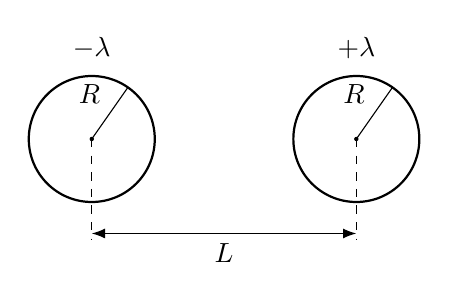
\begin{tikzpicture}[>=Latex,scale=.8]

 \draw[thick](-2.1,0)circle(1)(2.1,0)circle(1);
 \fill(-2.1,0)circle(1pt);\fill(2.1,0)circle(1pt);
 \draw(-2.1,0)--++(55:1)node[midway,above left]{$R$};\draw(2.1,0)--++(55:1)node[midway,above left]{$R$};
 \draw[dashed](-2.1,0)--(-2.1,-1.6)(2.1,0)--(2.1,-1.6);
 \draw[<->](-2.1,-1.5)--(2.1,-1.5)node[midway,below]{$L$};
 \node at(-2.1,1.45){$-\lambda$};\node at(2.1,1.45){$+\lambda$};

\end{tikzpicture}\end{center}
\figcap{无穷长平行导体圆柱的横截面，半径与圆心距如图。}\label{fig:em-source-thirty-fifth-section-3}
\end{origexamplebox}

\twoCylindersFigure
\diagramcaption{图 4.13：例题4.3。两圆柱截面是双极坐标中的两条等坐标圆。}

\begin{xesolution}
先说明为什么圆柱截面可由两条虚拟线电荷构造。令 $d=L/2$、$a=\sqrt{d^2-R^2}$，
在图4.13中 $x=\pm a$ 放虚拟线电荷 $\pm\lambda$。它们位于各自圆柱内部，
只在柱外使用对应电势 $\varphi=(\lambda/2\pi\varepsilon_0)\ln(r_-/r_+)$。
取 $\xi=\ln(r_-/r_+)$ 为常量，配方得到圆心 $a\coth\xi$、半径 $a/|\sinh\xi|$；
因此选择 $\cosh\xi_0=d/R$ 就恰好得到两条真实圆柱边界。
每柱外围的高斯面包围一根虚拟线电荷，故计算出的 $\lambda$ 就是真实单位长度总电荷。

这是二维静电问题。采用双极坐标 $(\xi,\eta)$，其尺度因子为
\[
 h_\xi=h_\eta=\frac a{\cosh\xi-\cos\eta}.
\]
两个圆柱面可取为 $\xi=\pm\xi_0$。由双极坐标几何关系
\[
 R=\frac a{\sinh\xi_0},\qquad
 \frac L2=a\coth\xi_0,
\]
消去 $a$ 得
\[
 \cosh\xi_0=\frac{L}{2R},\qquad
 \xi_0=\operatorname{arcosh}\frac{L}{2R}.
\]
令两柱电势分别为 $+U/2$ 和 $-U/2$。满足 Laplace 方程及边界条件的电势是
\[
 \varphi(\xi)=\frac{U}{2\xi_0}\xi.
\]
在 $\xi=\xi_0$ 的圆柱面上，法向电场大小
$E_n=(1/h_\xi)\,\partial\varphi/\partial\xi$，弧元为
$\mathrm ds=h_\eta\mathrm d\eta$。因此单位长度电荷量
\[
 \lambda=\varepsilon_0\int_0^{2\pi}E_n\,\mathrm ds
 =\varepsilon_0\int_0^{2\pi}\frac{U}{2\xi_0}\,\mathrm d\eta
 =\frac{\pi\varepsilon_0U}{\xi_0}.
\]
单位长度电容为
\[
 \boxed{C'=\frac\lambda U
 =\frac{\pi\varepsilon_0}{\operatorname{arcosh}(L/2R)}
 =\frac{\pi\varepsilon_0}
 {\ln\!\left[\dfrac{L+\sqrt{L^2-4R^2}}{2R}\right]}}.
\]
当 $L\gg R$ 时，$C'\simeq\pi\varepsilon_0/\ln(L/R)$。
\end{xesolution}

\Needspace{10\baselineskip}
\begin{origexamplebox}{例题 4.4【改造电容器】}
如图，一个平行板电容器的极板面积为 $S$、间距为 $d$。

(1) 在左边一半插入相对介电常数为 $\varepsilon_r$ 的介质，电容变为多大？变大还是变小？

(2) 在上边一半插入相对介电常数为 $\varepsilon_r$ 的介质，电容变为多大？变大还是变小？
\emModifiedQuestion\figcap{介质分别占一半正对面积或一半板间厚度。}\label{fig:em-modified-question}
\end{origexamplebox}

图 4.14 左图的两部分共有相同板间电压；右图的两层沿电场方向依次排列，分别对应并联与串联。

\modifiedCapacitorFigure
\diagramcaption{图 4.14：例题4.4。左图按面积分区，应视为并联；右图按厚度分层，应视为串联。}

\begin{xesolution}
原电容为 $C_0=\varepsilon_0S/d$。

\textbf{(1) 按面积分区。} 两个区域的电势差均为同一个 $U$，相当于并联：
\[
 C_1=\varepsilon_r\varepsilon_0\frac{S/2}{d},\qquad
 C_2=\varepsilon_0\frac{S/2}{d}.
\]
故
\[
 \boxed{C=C_1+C_2=\frac{\varepsilon_r+1}{2}C_0}.
\]

\textbf{(2) 按厚度分层。} 电场依次穿过厚度均为 $d/2$ 的介质层和真空层，自由面电荷相同，相当于串联：
\[
 C_1=\varepsilon_r\varepsilon_0\frac S{d/2}=2\varepsilon_rC_0,
 \qquad C_2=\varepsilon_0\frac S{d/2}=2C_0.
\]
所以
\[
 \boxed{C=\frac{C_1C_2}{C_1+C_2}
 =\frac{2\varepsilon_r}{\varepsilon_r+1}C_0}.
\]
因为 $\varepsilon_r>1$，两种改造都使电容增大；但两者通常不相等。判断“并联还是串联”的依据不是
图画在左边还是上边，而是各区域共享电压还是依次承受电压。
\end{xesolution}

\Needspace{11\baselineskip}
\begin{origexamplebox}{例题 4.5【奇妙的吸引力】}
把相对介电常数为 $\varepsilon_r$ 的电介质部分插入平行板电容器。极板长为 $a$、宽为 $b$、间距为
$d$，介质插入长度为 $x$，如图。利用虚功法求介质受到的力：

(1) 电容器电荷 $Q$ 恒定；

(2) 电容器接在电压为 $U$ 的理想电源上。

两问均用电容器内的电场 $E$ 表示结果。
\emInsertionQuestion\figcap{介质插入长度与电容器尺寸；受力方向待求。}\label{fig:em-insertion-question}
\end{origexamplebox}

图 4.15 中 $x$ 向右增加，表示介质插入更深；因此由能量求得的正 $F$ 指向右。

\dielectricInsertionFigure
\diagramcaption{图 4.15：例题4.5。介质区和真空区并联，电场方向竖直，吸引力沿插入方向。}

\begin{xesolution}
忽略边缘场。插入部分与未插入部分共享相同板间电压，因此
\[
 C(x)=\varepsilon_r\varepsilon_0\frac{bx}{d}
      +\varepsilon_0\frac{b(a-x)}d
 =\frac{\varepsilon_0b}{d}\bigl[a+(\varepsilon_r-1)x\bigr],
\]
从而
\[
 \frac{\mathrm dC}{\mathrm dx}
 =\frac{\varepsilon_0b}{d}(\varepsilon_r-1)>0.
\]

\textbf{(1) 定电荷。} 电容场能 $W=Q^2/(2C)$，虚位移 $\mathrm dx$ 时
\[
 F=-\frac{\mathrm dW}{\mathrm dx}
 =\frac{Q^2}{2C^2}\frac{\mathrm dC}{\mathrm dx}.
\]
又 $Q/C=U=Ed$，故
\[
 \boxed{F=\frac12\varepsilon_0(\varepsilon_r-1)b d\,E^2}.
\]

\textbf{(2) 定电压。} 电容器本身的场能是 $CU^2/2$，但介质移动时电源还要搬运电荷
$\mathrm dQ=U\,\mathrm dC$。把电容器与电源作为整体，其与机械坐标有关的势能是
\[
 \mathcal G=\frac12CU^2-UQ=-\frac12CU^2.
\]
因此
\[
 F=-\frac{\mathrm d\mathcal G}{\mathrm dx}
 =\frac12U^2\frac{\mathrm dC}{\mathrm dx}
 =\boxed{\frac12\varepsilon_0(\varepsilon_r-1)b d\,E^2}.
\]
两问用瞬时场强 $E$ 表示时形式相同，方向都指向增大 $x$ 的方向，即介质被吸入电容器。定电压情形若
遗漏电源做功，会错误地得到相反的力。
\end{xesolution}

\Needspace{9\baselineskip}
\begin{origexamplebox}{例题 4.6【匀强电场中的电介质球】}
半径为 $R$、相对介电常数为 $\varepsilon_r$ 的电介质球放在匀强电场
$\boldsymbol E_0=E_0\hat{\boldsymbol z}$ 中，求空间中的电场。
\end{origexamplebox}

\dielectricSphereFieldFigure
\diagramcaption{解图：$\varepsilon_r=4$ 时的电介质球，$+z$ 沿外场。线表示场的方向，线密度不用于跨介质比较 $E$ 的大小；界面处切向 $E$、法向 $D$ 连续。}

\begin{xesolution}
问题关于 $z$ 轴对称，且远处电势应趋于 $-E_0r\cos\theta$。球内电势在原点必须有限，球外附加项
必须在无穷远消失，因此设
\[
 \varphi_{\rm in}=-Ar\cos\theta,
 \qquad
 \varphi_{\rm out}=-E_0r\cos\theta+\frac{B\cos\theta}{r^2}.
\]
球面 $r=R$ 上没有自由面电荷，故电势连续、法向电位移连续：
\[
 \varphi_{\rm in}=\varphi_{\rm out},\qquad
 \varepsilon_r\varepsilon_0E_{r,\rm in}=\varepsilon_0E_{r,\rm out}.
\]
比较两侧 $\cos\theta$ 的系数，第一条边界条件给出 $A=E_0-B/R^3$；
由 $E_r=-\partial\varphi/\partial r$，第二条给出
$\varepsilon_r A=E_0+2B/R^3$。将第一式代入第二式：
\[
 (\varepsilon_r+2)\frac B{R^3}=(\varepsilon_r-1)E_0.
\]
再回代即得
\[
 A=\frac{3E_0}{\varepsilon_r+2},\qquad
 B=\frac{\varepsilon_r-1}{\varepsilon_r+2}E_0R^3.
\]
所以球内电场为
\[
 \boxed{\boldsymbol E_{\rm in}=\frac{3}{\varepsilon_r+2}\boldsymbol E_0}.
\]
球外电场分量为
\[
 \boxed{\begin{aligned}
 E_r&=E_0\cos\theta+
 2\frac{\varepsilon_r-1}{\varepsilon_r+2}E_0\frac{R^3}{r^3}\cos\theta,\\
 E_\theta&=-E_0\sin\theta+
 \frac{\varepsilon_r-1}{\varepsilon_r+2}E_0\frac{R^3}{r^3}\sin\theta.
 \end{aligned}}
\]
附加项正是位于球心、方向沿 $\boldsymbol E_0$ 的偶极子场。等效偶极矩为
\[
 \boldsymbol p_{\rm eff}=4\pi\varepsilon_0R^3
 \frac{\varepsilon_r-1}{\varepsilon_r+2}\boldsymbol E_0.
\]
\end{xesolution}

\Needspace{8\baselineskip}
\begin{origexamplebox}{例题 4.7【能量怎么多了】}
线性电介质中的电场能量密度为
$u=\tfrac12\varepsilon_r\varepsilon_0E^2$，而真空中在相同场强下只有
$u_0=\tfrac12\varepsilon_0E^2$。试提出一个物理图像解释这个现象。
\end{origexamplebox}

\polarizationEnergyFigure
\diagramcaption{解图：极化可类比为微观正负电荷之间的“弹簧”被拉伸；建立同样场强时还要为极化自由度输入能量。}

\begin{xesolution}
线性介质中
\[
 \boldsymbol D=\varepsilon_0\boldsymbol E+\boldsymbol P,
 \qquad
 u=\frac12\boldsymbol E\cdot\boldsymbol D
 =\frac12\varepsilon_0E^2+\frac12\boldsymbol E\cdot\boldsymbol P.
\]
第一项是真空电场能；第二项是建立极化时外界对束缚正、负电荷做功所对应的能量。可以把原子内部的
正负电荷中心想成由微观弹性约束连接：外场把它们拉开，形成偶极矩，同时在材料的极化自由度中储存
能量。因此在\emph{相同实际场强 $E$} 下，介质比真空多出
\[
 u-u_0=\frac12\boldsymbol E\cdot\boldsymbol P
 =\frac12(\varepsilon_r-1)\varepsilon_0E^2.
\]
这并不意味着插入介质后能量一定增加。若自由电荷 $Q$ 固定，插入介质使 $E$ 减小，电容器总能量
$Q^2/(2C)$ 反而降低，差值转化为机械功；若电压固定，电源继续输送电荷，场能增加，增加的能量来自
电源。必须先说明固定的是 $E$、$Q$ 还是 $U$。
\end{xesolution}

\Needspace{10\baselineskip}
\begin{origexamplebox}{例题 4.8【充电过程】}
用电动势为 $\mathcal E$ 的电源给电容 $C$ 充电。

(1) 若电路中有电阻 $R$，直至充电完成，电源做功多少，发热多少？

(2) 若电阻 $R\to0^+$，电源做功多少，发热多少？

(3) 如果电路中完全没有电阻，答案会有什么变化？
\end{origexamplebox}

\chargingEnergyFigure
\diagramcaption{解图：理想恒压源经任意正电阻给电容充电时，电源做功的一半进入电场，另一半成为焦耳热。}

\begin{xesolution}
充电完成后 $Q=C\mathcal E$。电源每搬运电量 $\mathrm dq$ 做功
$\mathcal E\,\mathrm dq$，所以总功
\[
 W_{\rm s}=\int_0^Q\mathcal E\,\mathrm dq
 =\mathcal EQ=C\mathcal E^2.
\]
电容器最终储能
\[
 W_C=\frac12C\mathcal E^2.
\]
由能量守恒，电阻发热
\[
 \boxed{Q_R=W_{\rm s}-W_C=\frac12C\mathcal E^2}.
\]

也可直接积分验证。$RC$ 电路电流
$i(t)=(\mathcal E/R)e^{-t/(RC)}$，因此
\[
 Q_R=\int_0^\infty i^2R\,\mathrm dt
 =\frac{\mathcal E^2}{R}\int_0^\infty e^{-2t/(RC)}\,\mathrm dt
 =\frac12C\mathcal E^2.
\]
结果与 $R$ 的大小无关。故 $R\to0^+$ 时，充电时间趋于零、瞬时功率趋于无穷，但积分后的电源功和
发热仍分别为 $C\mathcal E^2$ 与 $C\mathcal E^2/2$。

若令 $R$ \emph{严格等于零}，同时又把电感、辐射和电源内阻全部忽略，理想模型在接通瞬间要求电容
电压跳变并产生冲激电流，问题本身不再自洽。真实电路总有电感或辐射损耗；若只保留电感 $L$ 而没有
任何耗散，系统会发生 $LC$ 振荡，电容也不会不可逆地停在“充电完成”状态。因此第(2)问的极限不能
简单替代第(3)问的严格零电阻模型。
\end{xesolution}

\Needspace{9\baselineskip}
\begin{origexamplebox}{例题 4.9【电容充电】}
如图，三个电容器初始均不带电，连接成 $Y$ 型，三条外支路的电势分别为
$\varphi_1,\varphi_2,\varphi_3$。求三个电容器外侧极板所带电荷。
\yCapacitorFigure
\diagramcaption{图 4.16：例题4.9。三个电容器的内侧极板连接成一个浮置中性节点。}
\end{origexamplebox}

图 4.16 的三个内侧极板连接在同一节点上，电势均为 $V$；该节点与外界不导通，所以其总电荷保持为零。



\begin{xesolution}
设中心浮置节点电势为 $V$。第 $i$ 个电容器外侧极板的电荷为
\[
 q_i=C_i(\varphi_i-V).
\]
中心节点由三个内侧极板和连接导线组成，初始净电荷为零，又与外界绝缘，所以始终满足
\[
 \sum_{i=1}^3C_i(V-\varphi_i)=0.
\]
由此
\[
 \boxed{V=\frac{C_1\varphi_1+C_2\varphi_2+C_3\varphi_3}
 {C_1+C_2+C_3}}.
\]
代回得
\[
 \boxed{q_i=C_i\left(\varphi_i-
 \frac{\sum_jC_j\varphi_j}{\sum_jC_j}\right)}.
\]
显式写出例如
\[
 q_1=\frac{C_1}{C_1+C_2+C_3}
 \bigl[C_2(\varphi_1-\varphi_2)+C_3(\varphi_1-\varphi_3)\bigr],
\]
其余两式循环置换指标即可。可检查 $q_1+q_2+q_3=0$，这与整个三电容系统初始总电荷为零一致。
\end{xesolution}

\Needspace{9\baselineskip}
\begin{origexamplebox}{例题 4.10【电容串并联】}
证明两个电容器串联或并联时都可以等效成一个电容器，求出等效公式，并讨论更多电容器串、并联时
是否也可以等效。
\end{origexamplebox}

\begin{xesolution}
等效的含义是：从外部两个端口看，在任意端电压 $U$ 下，系统从电源取得的总电荷 $Q$ 与某个单电容
$C_{\rm eq}$ 完全相同，即 $Q=C_{\rm eq}U$。

\textbf{并联：} 各电容两端电压均为 $U$，总电荷
\[
 Q=\sum_iQ_i=\sum_iC_iU,
\]
故
\[
 \boxed{C_{\rm eq}=\sum_iC_i}.
\]

\textbf{串联：} 每个中间浮置节点初始净电荷为零，因此各电容器电荷量大小均为 $Q$。总电压
\[
 U=\sum_iU_i=Q\sum_i\frac1{C_i},
\]
故
\[
 \boxed{\frac1{C_{\rm eq}}=\sum_i\frac1{C_i}}.
\]
结论可直接推广到任意多个纯并联或纯串联电容。由串、并联组成的两端网络可逐级化简；更一般的线性
两端电容网络，只要内部节点初始无净电荷，也存在一个等效电容，但未必能只用一次串并联公式求出，
需要先列内部节点电荷守恒方程。若网络有三个以上独立外端口，则通常需要电容系数矩阵，不能用一个
标量电容完整描述。
\end{xesolution}

\Needspace{12\baselineskip}
\begin{origexamplebox}{例题 4.11【超大电容】}
Kelvin 曾把大气层构造为一个电容器模型：地球表面是一个极板，带有
$5\times10^5\,\mathrm C$ 的负电荷；把距地表 $5\,\mathrm{km}$ 的同心球面作为带正电的等效外极板，两极之间的大气层厚度为 $5\,\mathrm{km}$。

(1) 求这个球形电容器的电容；

(2) 求地球表面的电场能量密度以及球形电容器的总能量；

(3) 已知空气电阻率为 $3\times10^{13}\,\Omega\!\cdot\!\mathrm m$，求两极间大气层的电阻；

(4) 大气电容与电阻构成 $RC$ 放电回路，求时间常数；

(5) 若平均一次雷电向地面补充 $25\,\mathrm C$ 电荷，为维持上述电荷量，全球每天平均需要多少次雷电？
\end{origexamplebox}

\earthCapacitorFigure
\diagramcaption{解图：地球表面与高空等效层构成同心球形电容器；大气同时提供漏电电阻。}

\begin{xesolution}
取地球半径 $R_\oplus=6.4\times10^6\,\mathrm m$，大气等效厚度
$d=5.0\times10^3\,\mathrm m$，外层半径 $R_\oplus+d$，电荷量大小
$Q=5.0\times10^5\,\mathrm C$。

\textbf{(1) 电容。} 同心球形电容公式给出
\[
 C=4\pi\varepsilon_0\frac{R_\oplus(R_\oplus+d)}d
 \simeq4\pi\varepsilon_0\frac{R_\oplus^2}{d}
 =\boxed{0.912\,\mathrm F}.
\]

\textbf{(2) 能量密度与总能量。} 地表场强
\[
 E(R_\oplus)=\frac{Q}{4\pi\varepsilon_0R_\oplus^2}
 \simeq1.10\times10^2\,\mathrm{V/m}.
\]
故地表能量密度
\[
 \boxed{u(R_\oplus)=\frac12\varepsilon_0E^2
 \simeq5.33\times10^{-8}\,\mathrm{J/m^3}}.
\]
总能量
\[
 \boxed{W=\frac{Q^2}{2C}\simeq1.37\times10^{11}\,\mathrm J}.
\]
相应电势差约为 $U=Q/C\simeq5.48\times10^5\,\mathrm V$。

\textbf{(3) 大气电阻。} 径向电流通过半径 $r$ 处面积 $4\pi r^2$，微元电阻
$\mathrm dR=\rho\,\mathrm dr/(4\pi r^2)$，因此
\[
 R_{\rm air}=\frac\rho{4\pi}
 \left(\frac1{R_\oplus}-\frac1{R_\oplus+d}\right)
 =\boxed{2.91\times10^2\,\Omega}.
\]

\textbf{(4) 时间常数。} 两个球壳使用完全相同的几何因子，故
\[
 \tau=R_{\rm air}C=\rho\varepsilon_0
 =\boxed{2.66\times10^2\,\mathrm s}\approx4.43\,\mathrm{min}.
\]

\textbf{(5) 雷电次数。} 为维持近似恒定的 $Q$，平均补充电流需抵消漏电流
$I=Q/\tau$。一天需要补充的电荷为 $Q(86400\,\mathrm s)/\tau$，所以
\[
 N=\frac{Q}{\tau}\frac{86400}{25}
 \simeq\boxed{6.5\times10^6\ \text{次/天}}.
\]
这个数值是题设均匀电阻率和固定等效高度模型的预测，不能单凭它认定真实全球雷电次数或验证大气电路。
真实电导率随高度变化，雷暴供电机制与单次输送电荷也有分布；本模型用于说明电容储能与漏电并存时的收支关系。
\end{xesolution}

\end{document}
